\documentclass{standalone}
\usepackage{tikz} 

\begin{document}

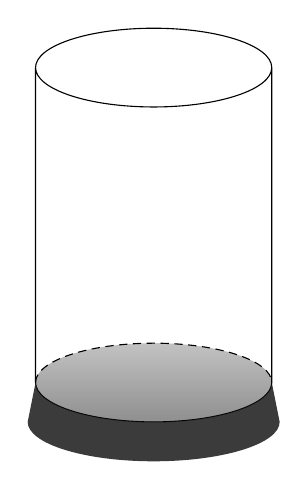
\begin{tikzpicture}
\fill[top color=gray!40, bottom color=black, shading=axis, opacity=0.25] (0,0) circle (1.5cm and 0.5cm); %bottom grayness
\draw (-1.5,4) -- (-1.5,0) arc (180:360:1.5cm and 0.5cm) -- (1.5,4) ++ (-1.5,0) circle (1.5cm and 0.5cm); %bottom front circle
\draw[densely dashed] (-1.5,0) arc (180:0:1.5cm and 0.5cm); %bottom back dashed circle

\fill[color=black!90, opacity=0.85] (-1.6,-0.5) -- (-1.5,0) arc (180:360:1.5cm and 0.5cm) -- (1.6,-0.5) arc (180:360:-1.6cm and 0.5cm); %base front circle

\fill[color=black!90, opacity=0.85] ; %handle

\end{tikzpicture} 

\end{document}